% ========================================
%	Header einbinden
% ========================================

\documentclass[bibtotoc,titlepage]{scrartcl}

% Deutsche Spracheinstellungen
\usepackage[ngerman,german]{babel, varioref}
\usepackage[T1]{fontenc}
\usepackage[utf8]{inputenc}

%\usepackage{marvosym}

\usepackage{amsfonts}
\usepackage{amssymb}
\usepackage{amsmath}
\usepackage{amscd}
\usepackage{amstext}

\usepackage{longtable}

%\usepackage{bibgerm}

\usepackage{footnpag}

\usepackage{ifthen}                 %%% package for conditionals in TeX
\usepackage[amssymb]{SIunits}
%Für textumflossene Bilder und Tablellen
%\usepackage{floatflt} - veraltet

%Für Testzwecke aktivieren, zeigt labels und refs im Text an.
%\usepackage{showkeys}

% Abstand zwischen zwei Absätzen nach DIN (1,5 Zeilen)
% \setlength{\parskip}{1.5ex plus0.5ex minus0.5ex}

% Einrückung am Anfang eines neuen Absatzes nach DIN (keine)
%\setlength{\parindent}{0pt}

% Ränder definieren
% \setlength{\oddsidemargin}{0.3cm}
% \setlength{\textwidth}{15.6cm}

% bessere Bildunterschriften
%\usepackage[center]{caption2}


% Problemlösungen beim Umgang mit Gleitumgebungen
\usepackage{float}

% Nummeriert bis zur Strukturstufe 3 (also <section>, <subsection> und <subsubsection>)
%\setcounter{secnumdepth}{3}

% Führt das Inhaltsverzeichnis bis zur Strukturstufe 3
%\setcounter{tocdepth}{3}
\usepackage[version=3]{mhchem}
	\mhchemoptions{minus-sidebearing-left=0.06em, minus-sidebearing-right=0.11em}
\usepackage{exscale}

\newenvironment{dsm} {\begin{displaymath}} {\end{displaymath}}
\newenvironment{vars} {\begin{center}\scriptsize} {\normalsize \end{center}}


\newcommand {\en} {\varepsilon_0}               % Epsilon-Null aus der Elektrodynamik
\newcommand {\lap} {\; \mathbf{\Delta}}         % Laplace-Operator
\newcommand {\R} { \mathbb{R} }                 % Menge der reellen Zahlen
\newcommand {\e} { \ \mathbf{e} }               % Eulersche Zahl
\renewcommand {\i} { \mathbf{i} }               % komplexe Zahl i
\newcommand {\N} { \mathbb{N} }                 % Menge der nat. Zahlen
\newcommand {\C} { \mathbb{C} }                 % Menge der kompl. Zahlen
\newcommand {\Z} { \mathbb{Z} }                 % Menge der kompl. Zahlen
\newcommand {\limi}[1]{\lim_{#1 \rightarrow \infty}} % Limes unendlich
\newcommand {\sumi}[1]{\sum_{#1=0}^\infty}
\newcommand {\rot} {\; \mathrm{rot} \,}         % Rotation
\newcommand {\grad} {\; \mathrm{grad} \,}       % Gradient
\newcommand {\dive} {\; \mathrm{div} \,}        % Divergenz
\newcommand {\dx} {\; \mathrm{d} }              % Differential d
\newcommand {\cotanh} {\; \mathrm{cotanh} \,}   %Cotangenshyperbolicus
\newcommand {\asinh} {\; \mathrm{areasinh} \,}  %Area-Sinus-Hyp.
\newcommand {\acosh} {\; \mathrm{areacosh} \,}  %Area-Cosinus-H.
\newcommand {\atanh} {\; \mathrm{areatanh} \,}  %Area Tangens-H.
\newcommand {\acoth} {\; \mathrm{areacoth} \,}  % Area-cotangens
\newcommand {\Sp} {\; \mathrm{Sp} \,}
\newcommand {\mbe} {\stackrel{\text{!}}{=}}     %Must Be Equal
\newcommand{\qed} { \hfill $\square$\\}
\renewcommand{\i} {\imath}
\def\captionsngerman{\def\figurename{\textbf{Abb.}}}

%%%%%%%%%%%%%%%%%%%%%%%%%%%%%%%%%%%%%%%%%%%%%%%%%%%%%%%%%%%%%%%%%%%%%%%%%%%%
% SWITCH FOR PDFLATEX or LATEX
%%%%%%%%%%%%%%%%%%%%%%%%%%%%%%%%%%%%%%%%%%%%%%%%%%%%%%%%%%%%%%%%%%%%%%%%%%%%
%%%
\ifx\pdfoutput\undefined %%%%%%%%%%%%%%%%%%%%%%%%%%%%%%%%%%%%%%%%% LATEX %%%
%%%
\usepackage[dvips]{graphicx}       %%% graphics for dvips
\DeclareGraphicsExtensions{.eps,.ps}   %%% standard extension for included graphics
\usepackage[ps2pdf]{thumbpdf}      %%% thumbnails for ps2pdf
\usepackage[ps2pdf,                %%% hyper-references for ps2pdf
bookmarks=true,%                   %%% generate bookmarks ...
bookmarksnumbered=true,%           %%% ... with numbers
hypertexnames=false,%              %%% needed for correct links to figures !!!
breaklinks=true,%                  %%% breaks lines, but links are very small
linkbordercolor={0 0 1},%          %%% blue frames around links
pdfborder={0 0 112.0}]{hyperref}%  %%% border-width of frames
%                                      will be multiplied with 0.009 by ps2pdf
%
\hypersetup{ pdfauthor   = {Hannes Franke; Julius Tilly},
pdftitle    = {V301 Innenwiderstand und Leistungsanpassung}, pdfsubject  = {Protokoll FP}, pdfkeywords = {V301, Innenwiderstand, Leistungsanpassung},
pdfcreator  = {LaTeX with hyperref package}, pdfproducer = {dvips
+ ps2pdf} }
%%%
\else %%%%%%%%%%%%%%%%%%%%%%%%%%%%%%%%%%%%%%%%%%%%%%%%%%%%%%%%%% PDFLATEX %%%
%%%
\usepackage[pdftex]{graphicx}      %%% graphics for pdfLaTeX
\DeclareGraphicsExtensions{.pdf}   %%% standard extension for included graphics
\usepackage[pdftex]{thumbpdf}      %%% thumbnails for pdflatex
\usepackage[pdftex,                %%% hyper-references for pdflatex
bookmarks=true,%                   %%% generate bookmarks ...
bookmarksnumbered=true,%           %%% ... with numbers
hypertexnames=false,%              %%% needed for correct links to figures !!!
breaklinks=true,%                  %%% break links if exceeding a single line
linkbordercolor={0 0 1},
linktocpage]{hyperref} %%% blue frames around links
%                                  %%% pdfborder={0 0 1} is the default
\hypersetup{
pdftitle    = {V301 Innenwiderstand und Leistungsanpassung}, 
pdfsubject  = {Protokoll AP}, 
pdfkeywords = {V301, Innenwiderstand, Leistungsanpassung},
pdfsubject  = {Protokoll AP},
pdfkeywords = {V301, Innenwiderstand, Leistungsanpassung}}
%                                  %%% pdfcreator, pdfproducer,
%                                      and CreationDate are automatically set
%                                      by pdflatex !!!
\pdfadjustspacing=1                %%% force LaTeX-like character spacing
\usepackage{epstopdf}
%
\fi %%%%%%%%%%%%%%%%%%%%%%%%%%%%%%%%%%%%%%%%%%%%%%%%%%% END OF CONDITION %%%
%%%%%%%%%%%%%%%%%%%%%%%%%%%%%%%%%%%%%%%%%%%%%%%%%%%%%%%%%%%%%%%%%%%%%%%%%%%%
% seitliche Tabellen und Abbildungen
%\usepackage{rotating}
\usepackage{ae}
\usepackage{
  array,
  booktabs,
  dcolumn
}
\makeatletter 
  \renewenvironment{figure}[1][] {% 
    \ifthenelse{\equal{#1}{}}{% 
      \@float{figure} 
    }{% 
      \@float{figure}[#1]% 
    }% 
    \centering 
  }{% 
    \end@float 
  } 
  \makeatother 


  \makeatletter 
  \renewenvironment{table}[1][] {% 
    \ifthenelse{\equal{#1}{}}{% 
      \@float{table} 
    }{% 
      \@float{table}[#1]% 
    }% 
    \centering 
  }{% 
    \end@float 
  } 
  \makeatother 
%\usepackage{listings}
%\lstloadlanguages{[Visual]Basic}
%\allowdisplaybreaks[1]
%\usepackage{hycap}
%\usepackage{fancyunits}




% ========================================
%	Angaben für das Titelblatt
% ========================================

\title{Versuch 504 - Thermische Elektronenemission\\				% Titel des Versuchs 
\large TU Dortmund, Fakultät Physik\\ 
\normalsize Anfänger-Praktikum}

\author{Jan Adam\\			% Name Praktikumspartner A
{\small \href{jan.adam@tu-dortmund.de}{jan.adam@tu-dortmund.de}}	% Erzeugt interaktiven einen Link
\and						% um einen weiteren Author hinzuzfügen
Dimitrios Skodras\\					% Name Praktikumspartner B
{\small \href{dimitrios.skodras@tu-dortmund.de}{dimitrios.skodras@tu-dortmund.de}}		% Erzeugt interaktiven einen Link
}
\date{22.Januar 2013}				% Das Datum der Versuchsdurchführung

% ========================================
%	Das Dokument beginnt
% ========================================

\begin{document}

% ========================================
%	Titelblatt erzeugen
% ========================================

\maketitle					% Jetzt wird die Titelseite erzeugt
\thispagestyle{empty} 				% Weder Kopfzeile noch Fußzeile

% ========================================
%	Der Vorspann
% ========================================

%\newpage					% Wenn Verzeichnisse auf einer neuen Seite beginnen sollen
%\pagestyle{empty}				% Weder Kopf- noch Fußzeile für Verzeichnisse

\tableofcontents

%\newpage					% eine neue Seite
%\thispagestyle{empty}				% Weder Kopf- noch Fußzeile für Verzeichnisse
%\listoffigures					% Abbildungsverzeichnis

%\newpage					% eine neue Seite
%\thispagestyle{empty}				% Weder Kopf- noch Fußzeile für Verzeichnisse
%\listoftables					% Tabellenverzeichnis
\newpage					% eine neue Seite


% ========================================
%	Kapitel
% ========================================

\section{Einleitung}
Bei Metallen sind die äußeren Hüllenelektronen nur schwach an ihren Kern gebunden. Im kristallförmigen Gitter können sich die Elektronen daher nahezu frei bewegen, wodurch die gute elektrische Leitfähigkeit von Metallen erklärt wereden kann.
Erhält ein Elektron genügend Energie, um das nur noch schwache Kern-Potential zu überwinden, so kann es aus dem Metall austreten.
Erreichen kann man dies, indem man dem Elektron durch Stößen mit Photonen (Photoelektrischer Effekt) oder wie in diesem Versuch durch Erhöhung der Temperatur und somit ihrer thermischen Energie.

\section{Theorie}

\section{Durchführung}
\subsection{Versuchsaufbau}

\section{Auswertung}
\subsection{Kennlinienschar der Hochvakuumdiode}
Unter Anlegung von fünf verschiedenen Heizströmen $I_f$ wird die Beschleunigungsspannung $U_A$ erhöht und der fließende Strom $I_A$ 
gemessen. 

\begin{table}[H]
\begin{tabular}{|c|c||c|c||c|c||c|c||c|c|}
$I_f$ = 2,2 A & & $I_f$ = 2,4 A & & $I_f$ = 2,5 A & & $I_f$ = 2,6 A & & $I_f$ = 2,8 A&\\
\hline
$V_A$ & $I_A$ & $V_A$ & $I_A$ & $V_A$ & $I_A$ & $V_A$ & $I_A$ & $V_A$ & $I_A$\\
\hline
2&	3&	1&	3&	1&	5&	1&	5&	1&	6\\
3&	4&	2&	7&	2&	8&	2&	9&	2&	13\\
4&	6&	3&	10&	3&	12&	3&	15&	3&	18\\
5&	7&	4&	13&	4&	16&	4&	18&	4&	24\\
7&	8&	5&	16&	5&	20&	5&	24&	5&	29\\
8&	9&	6&	19&	6&	24&	6&	28&	6&	35\\
10&	10&	7&	22&	7&	28&	7&	33&	7&	40\\
12&	11&	8&	24&	8&	32&	8&	38&	8&	46\\
13&	11&	9&	27&	9&	35&	9&	42&	9&	52\\
15&	12&	10&	30&	10&	40&	10&	48&	10&	57\\
20&	14&	12&	35&	11&	44&	12&	60&	12&	72\\
25&	14&	15&	43&	12&	48&	14&	70&	14&	86\\
30&	15&	20&	54&	13&	53&	16&	83&	16&	103\\
35&	16&	25&	62&	14&	57&	18&	97&	18&	212\\
40&	16&	30&	68&	15&	61&	20&	110&	20&	139\\
50&	17&	35&	72&	20&	84&	22&	124&	22&	155\\
100&	19&	40&	75&	22&	92&	24&	138&	24&	172\\
125&	19&	50&	76&	25&	104&	25&	144&	25&	184\\
	& &	70&	79&	27&	109&	26&	151&	26&	193\\
	& &	90&	83&	30&	120&	28&	165&	28&	213\\
	& &	100&	85&	35&	133&	30&	177&	30&	233\\
	& &	150&	87&	40&	140&	35&	206&	32&	255\\
	& &		&&	45&	146&	40&	233&	34&	276\\
	& &		&&	50&	147&	45&	252&	36&	297\\
	& &		&&	60&	150&	50&	265&	38&	320\\
	& &		&&	70&	156&	55&	278&	40&	343\\
	&&		&&	80&	160&	60&	289&	45&	405\\
	&&		&&	90&	167&	70&	305&	50&	462\\
	&&		&&	100&	166&	80&	316&	55&	522\\
	&&		&&	150&	170&	90&	325&	60&	572\\
	&&		&&		&&	100&	332&	70&	680\\
	&&		&&		&&	150&	336&	80&	785\\
	&&		&&		&&		&&	90&	872\\
	&&		&&		&&		&&	100&	937\\
	&&		&&		&&		&&	110&	980\\
	&&		&&		&&		&&	120&	1010\\
	&&		&&		&&		&&	130&	1040\\
	&&		&&		&&		&&	140&	1060\\
	&&		&&		&&		&&	150&	1080\\
	&&		&&		&&		&&	200&	1130 \\
\hline
\end{tabular}
\label{tabheiz}
\caption{Beschleunigungsspannung $U_A$ und Strom $I_A$ zu fünf Heizströmen $I_f$}
\end{table}



\begin{figure}[H]
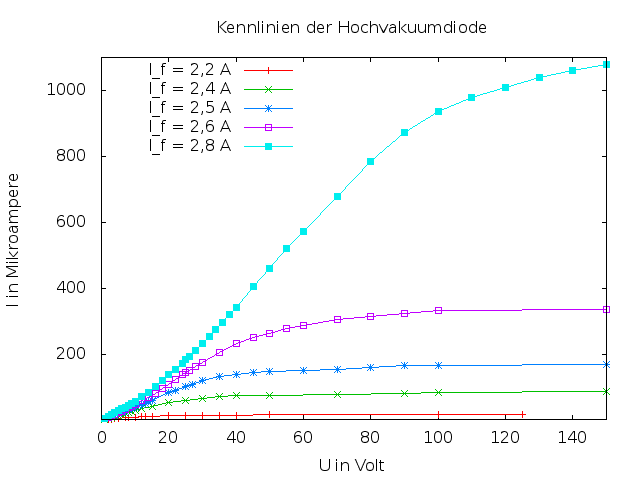
\includegraphics[width=0.8\textwidth]{pics/504a.png}
\end{figure}

\begin{figure}[H]
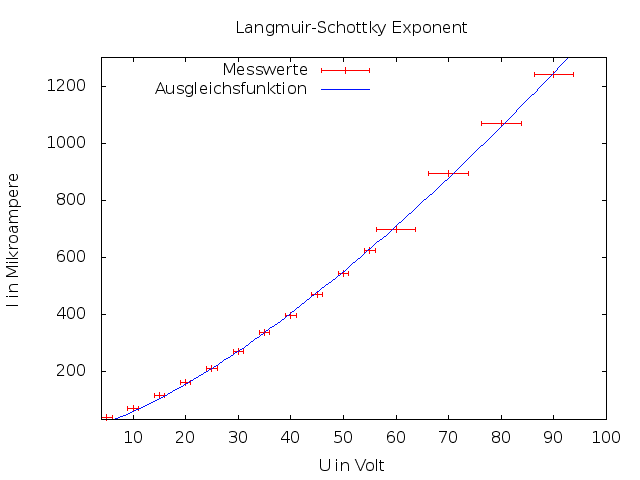
\includegraphics[width=0.8\textwidth]{pics/504b1.png}
\end{figure}

\begin{figure}[H]
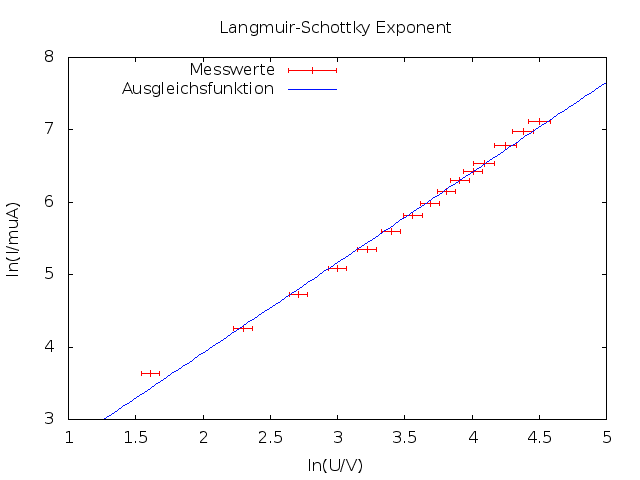
\includegraphics[width=0.8\textwidth]{pics/504b2.png}
\end{figure}

\begin{figure}[H]
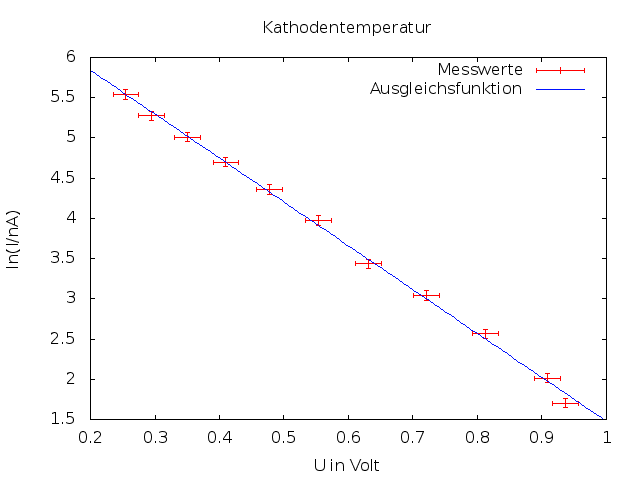
\includegraphics[width=0.8\textwidth]{pics/504c.png}
\end{figure}



\section{Diskussion}

% ========================================
%	Literaturverzeichnis
% ========================================

%\bibliographystyle{plainnat}			% Bibliographie-Style auswählen
%\bibliography{BIBDATEI}			% Literaturverzeichnis

% ========================================
%	Das Dokument endent
% ========================================

\end{document}
